%!TEX program = lualatex
\documentclass[10pt,mathserif]{beamer}

\usepackage{luatexja}
\usepackage{luatexja-fontspec}
\setmainjfont[
    RawFeature={instance=Regular},
    BoldFont=Noto Sans CJK SC,
    BoldFeatures={RawFeature={instance=Bold}},
]{Noto Sans CJK SC}

\setmonofont[
    RawFeature={instance=Regular},
    BoldFont=Noto Sans Mono,
    BoldFeatures={RawFeature={instance=Bold}},
]{Noto Sans Mono}

\definecolor{xdublue}{RGB}{0,65,130}

\usepackage{listings}
\lstset{
basicstyle=\small\ttfamily,
keywordstyle=\color{xdublue},
numbers=left,
numberstyle=\tiny,
frame=leftline,
tabsize=4
}

\lstdefinestyle{term}
{basicstyle=\ttfamily, numbers=none, frame=single, breaklines=true,
moredelim={[is][keywordstyle]{@@}{@@}}}

\newcommand{\lstcode}[1] { \lstinputlisting[language=C++]{code/#1} }
\newcommand{\lstterm}[1] { \lstinputlisting[style=term]{code/#1} }

\usepackage{ulem}

\usetheme[xdblue]{XDUstyle}

\title{Competitive Programming 101}
\institute{西安电子科技大学程序设计竞赛实训基地}
\author{席若尧}
\date{2021 年 7 月 5 日}
	
\begin{document}%
{\xdbg \frame[plain,noframenumbering]{\titlepage}}

\begin{frame}{内容}
	\tableofcontents[hideallsubsections]
\end{frame}

\section{ICPC 环境简介}
\sectionpage

\begin{frame}{基本认知}
	\begin{itemize}
		\item 程序设计竞赛与竞技体育/电子竞技类似
		\item 决定比赛成绩的因素有:天赋、训练、运气
		\item 不想训练的话也有很多低水平比赛可以打 (校赛,省赛,CSP 等)
		\item 想好好打的话,要对这项比赛有基本的认同感
		\item 尽量避免自视高贵/发表暴论
	\end{itemize}
\end{frame}

\begin{frame}{工作环境}
	\begin{itemize}
		\item Ubuntu GNU/Linux
			\begin{itemize}
				\item 没有 root 权限
			\end{itemize}
		\item GCC
		\item OpenJDK
		\item Python 3 or PyPy 3
		\item Vim, Emacs, Gedit, Code::Blocks 等
	\end{itemize}
\end{frame}

\begin{frame}{DOMJudge}
	\begin{itemize}
		\item 提交代码
		\item 打印代码
		\item 看榜
		\item 提问
	\end{itemize}
\end{frame}

\begin{frame}{团队配合}
	\begin{itemize}
		\item 三人一机
		\item 实力 (训练量) 是配合的基础
	\end{itemize}
\end{frame}

\section{程序的行为和编译优化}
\sectionpage

\begin{frame}{现状}
	\begin{itemize}
		\item 本节内容应该是程序设计基础课程的一部分,但是懂的都懂
	\end{itemize}
	\begin{center}
		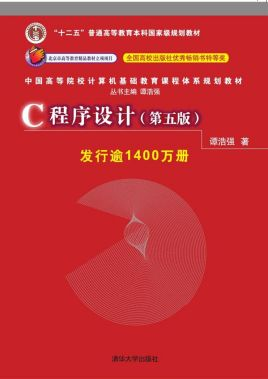
\includegraphics[width=.3\textwidth]{img/shit2.jpg}
	\end{center}
\end{frame}

\begin{frame}{现状}
	\begin{itemize}
		\item “你不确定的话就写个程序跑一下吧。”
			\pause
		\item 要是化学老师这么教课,实验室早炸上天了
	\end{itemize}
\end{frame}

\begin{frame}{现状}
	\begin{itemize}
		\item “我打了 3 年 OI 还能不知道自己的程序啥行为?”
			\pause
		\item 众所周知 NOIP 不开 \texttt{-O2}
	\end{itemize}
\end{frame}

\begin{frame}{程序的行为}
	C 标准 (\texttt{ISO/IEC 9899:2011} \S 5.1.2.3 p6) 规定,
	程序的\textbf{可观测行为}包括:
	\begin{itemize}
		\item 访问 \texttt{volatile} 变量
		\item 写入文件
		\item 操作交互式输入输出设备
	\end{itemize}
	实现 (在实践中由编译器和运行库组成) 只需要正确实现可观测行为。
	编译器可以在保证可观测行为不变的前提下,通过调整生成的机器代码,
	使得程序变得更小或更快。
\end{frame}

\begin{frame}[fragile]{例}{Hello world}
	\lstcode{hw.cc}
\end{frame}

\begin{frame}[fragile]{例}{Hello World}
	生成的汇编代码根本没有 \texttt{printf}?
	\lstinputlisting[style=term,emph={puts},emphstyle=\color{xdublue}]
	{code/hw.out}
\end{frame}

\begin{frame}[fragile]{例}{取模}
	\lstcode{mod.cc}
\end{frame}

\begin{frame}[fragile]{例}{取模}
	没有除法指令?
	\lstterm{mod.out}
\end{frame}

\begin{frame}[fragile]{例}{取模 (误)}
	\lstcode{mod_bad.cc}
\end{frame}

\begin{frame}[fragile]{例}{取模 (误)}
	\lstinputlisting[style=term,emph={idivl},emphstyle=\color{xdublue}]
	{code/mod_bad.out}
	\begin{itemize}
		\item 看上去简洁很多?
		\item 悲剧的是,这条除法指令比之前的一大堆加起来都慢。
		\item 实际做题时,因为忘加这个 \texttt{const},可能引入
			$50\%$ 至 $200\%$ 的时间代价。
	\end{itemize}
\end{frame}

\begin{frame}[fragile]{例}{strstr (Linux)}
	\lstcode{strstr.cc}
	\begin{itemize}
		\item 这题不用 KMP 能过?
	\end{itemize}
\end{frame}

\begin{frame}[fragile]{例}{strstr (Linux)}
	\lstterm{strstr.out}
	\begin{itemize}
		\item 在 Linux 上跑得飞快
		\item Glibc 的 \lstinline{strstr} 是时间
			$\mathcal{O}(n + m)$,空间 $\mathcal{O}(1)$ 的高级算法,
			而且是高度优化的手写汇编代码
	\end{itemize}
\end{frame}

\begin{frame}[fragile]{例}{strlen (运气好)}
	\lstcode{strlen-1.cc}
	\begin{itemize}
		\item 目测是 $\mathcal{O}(n^2)$ 的,会 TLE?
	\end{itemize}
\end{frame}

\begin{frame}[fragile]{例}{strlen (运气好)}
	\lstterm{strlen-1.out}
	\begin{itemize}
		\item 然而跑得飞快
	\end{itemize}
\end{frame}

\begin{frame}[fragile]{例}{strlen (运气差)}
	\lstcode{strlen-2.cc}
	\begin{itemize}
		\item 就改个大小写,不会出大问题吧
	\end{itemize}
\end{frame}

\begin{frame}[fragile]{例}{strlen (运气差)}
	\lstterm{strlen-2.out}
	\begin{itemize}
		\item 人都没了
		\item 编译器的能力是有极限的\sout{,所以我不做编译器辣!}
	\end{itemize}
\end{frame}

\begin{frame}{几类行为}
	\begin{itemize}
		\item 标准定义的行为
		\item 实现定义的行为 (implementation-defined)
		\item 未指定行为 (unspecified)
		\item 未定义行为 (undefined)
	\end{itemize}
\end{frame}

\begin{frame}[fragile]{实现定义的行为}
	标准要求实现作出一致的选择。
	\begin{itemize}
		\item 一个典型例子是 \lstinline{rand} 函数生成随机数的规则
			(包括但不限于 \lstinline{RAND_MAX} 的值),
			这在 2020 -- 2021 ICPC 区域赛南京站产生了显著的影响。
		\item 另一个例子是 FFT 等场合常用的卡常技巧
			\lstinline{a += M & (a >> 31);},它的目的是将
			$[-M, M)$ 中的整数模 $M$ (变为 $[0, M)$ 中的整数)。
			其正确性依赖于 GCC 规定负数右移按算术右移规则进行,
			如果更换编译器则可能出错。
	\end{itemize}
\end{frame}

\begin{frame}{未指定行为}
	标准未作说明,允许实现随意选择。
	\begin{itemize}
		\item 几乎所有程序都会涉及未指定行为,例如函数调用时,
			对其参数求值的顺序就是未指定的。
		\item 但是,如果你的 (比赛用) 程序的输出依赖于某个未指定行为,
			那么很有可能产生难以调试的 bug。
	\end{itemize}
\end{frame}

\begin{frame}[fragile]{例}
	\lstcode{unspecified.cc}
	\begin{itemize}
		\item 如果实现先对后一个 \lstinline{read()} 求值怎么办?
	\end{itemize}
\end{frame}

\begin{frame}[fragile]{修复}
	\lstcode{unspecified-fix.cc}
	\begin{itemize}
		\item 语言标准要求初始化列表中的元素必须从左到右求值。
	\end{itemize}
\end{frame}

\begin{frame}{未定义行为}
	\begin{itemize}
		\item 语法错误
		\item 语义错误
			\begin{itemize}
				\item 违反约束条件 (constraint):要求编译器将其视为编译错误
				\item 其他:未定义行为,实现可以干任何事!
			\end{itemize}
	\end{itemize}
\end{frame}

\begin{frame}{未定义行为}
	\begin{itemize}
		\item “什么都可能发生”
		\item 在没有操作系统或操作系统欠缺安全机制时,甚至能够损毁硬件
		\item 在比赛中可能产生“本地测不出来 bug,但交上去就错”的问题
	\end{itemize}
\end{frame}

\begin{frame}[fragile]{例}{函数无返回值}
	\begin{columns}[t]
		\begin{column}{.5\textwidth}
			\begin{itemize}
				\item 一类十分值得注意的未定义行为是,
					在非 \lstinline{void} 函数中,程序流程到达函数尾。
				\item 注意此时无论是否实际使用了该函数的返回值,
					只要程序执行到函数尾,都是未定义行为。
				\item 在编译器执行优化时,它可能假设
					“程序永远不会执行到该函数的尾部”,
					从而产生更加奇怪的行为。
				\item \textbf{老资格的 OI 选手}需要特别注意!
			\end{itemize}
		\end{column}
		\begin{column}{.5\textwidth}
			\lstcode{no-return.cc}
		\end{column}
	\end{columns}
\end{frame}

\begin{frame}{关于未定义行为}
	某些人总是无视语言标准尝试使用各种未定义行为,
	然后到处说“这程序在我的电脑上能工作,为什么交上去就错?”
	对此,Roger Miller 讽刺道:
	\begin{itemize}
		\item 有人曾经告诉我,在打篮球的时候,你不能带球走。
			我找了个篮球试了一下,发现走得很好。
			那人显然根本不懂篮球。
	\end{itemize}
	\pause
	\center
	
\includegraphics[width=2.5in]{img/cxk.jpg}
\end{frame}

\begin{frame}{没有银弹}
	\begin{center}
	\begin{tikzpicture}[fill=xdublue]
		\def\outbox{(-2, -2) rectangle(3, 3)}
		\def\firstcircle{(0, 0) circle(1)}
		\def\secondcircle{(1, 0) circle(1)}
		\def\thirdcircle{(0.5, 1) circle(1)}
		\fill[even odd rule]
		\outbox \firstcircle \secondcircle \thirdcircle;
		\draw \firstcircle node[left] {安全};
		\draw \secondcircle node[right] {高效};
		\draw \thirdcircle node[above] {易用};
		\draw \firstcircle node[shift={(-0.1,0.6)}]
		{\textcolor{white}{慢}};
		\draw \secondcircle node[shift={(0.1,0.6)}]
		{\textcolor{white}{\tiny 不安全}};
		\draw \thirdcircle node[shift={(0,-1.2)}]
		{\textcolor{white}{难学}};
		\draw \thirdcircle node[shift={(0,-0.6)}] {???};
		\draw \outbox node[shift={(-1,-1)}] {\textcolor{white}{屑}};
	\end{tikzpicture}
	\end{center}
\end{frame}

\section{常见编程错误}
\sectionpage

\begin{frame}{概述}
	\begin{itemize}
		\item 在比赛和实际工作中,总是会不可避免地写出错误 (或有瑕疵) 的代码
		\item 在软件开发中,通常要为系统测试和调试预留 $50\%$ 以上的时间
		\item 本节主要介绍现场赛可用的测试和调试手段,其他 (如 Valgrind 等) 可以自行了解
	\end{itemize}
\end{frame}

\subsection{评测系统返回的错误信息}

\begin{frame}{评测结果}
	首先介绍评测系统 (主要是 DOMJudge) 可能返回的错误信息:
	\begin{itemize}
		\item COMPILER-ERROR
		\item TIMELIMIT
		\item RUN-ERROR
		\item OUTPUT-LIMIT
		\item WRONG-ANSWER (以及 NO-OUTPUT)
	\end{itemize}
	再次强调:未定义行为可能导致评测返回任何一种错误!
\end{frame}

\begin{frame}{编译错误}{COMPILER-ERROR}
	\begin{itemize}
		\item 指你的程序无法编译成可执行文件
		\item 一般 OJ 都提供了查看编译器输出消息的方法,照着改即可
		\item 正式比赛要求选手机器和评测机完全一致,所以几乎不会出现
		\item 正式比赛 CE 不算罚时
	\end{itemize}
\end{frame}

\begin{frame}{时间超限}{TIMELIMIT}
	\begin{itemize}
		\item 你的程序跑得太慢了
	\end{itemize}
\end{frame}

\begin{frame}{运行错误}{RUN-ERROR}
	\begin{itemize}
		\item 你的程序没有以返回值 $0$ 正常退出
		\item 一般是因为出现了未定义行为
		\item 也可能是不小心返回了一个非 $0$ 值,比如压行压成了
			\lstinline{exit(printf("\%d\\n", x));}
		\item 现场赛使用 DOMJudge,内存超限也报告为运行错误
	\end{itemize}
\end{frame}

\begin{frame}{输出超限}{OUTPUT-LIMIT}
	\begin{itemize}
		\item 你输出了太多东西,超过了题目的限制 (DOMJudge 默认 $8$ MB)
		\item 可能是陷入了带输出的死循环
		\item 也可能是忘了删除调试输出 :)
		\item 对于某些题目只是 WA 的一种表现形式
			\begin{itemize}
				\item 例如:如果有解输出一个 $[0,9]$ 中的整数,
					如果无解输出
					\lstinline!"a very very long error message"!,
					那么如果把很多有解的情况判断成了无解就可能输出超限
			\end{itemize}
	\end{itemize}
\end{frame}

\begin{frame}{答案错误}{WRONG-ANSWER}
	\begin{itemize}
		\item 你的程序输出和标准答案不一致,或者被 SPJ 判断为错误
		\item 不同评测系统对于空白字符 (特别是行末空格和文末回车)
			的处理不一致,如果空白字符有区别可能返回 AC、WA、PE 等不同结果。
		\item DOMJudge 没有 PE,无 SPJ 的情况下会忽略行末空格和文末回车,
			但对于空白字符的其他差异会直接返回 WA。
			建议写输出时遵循一般的规范,每行都以 \lstinline!"\\n"! 结束,
			行末不要有多余的空格
		\item 如果完全没有输出,一些评测系统 (包括 DOMJudge) 会返回
			\lstinline{"NO-OUTPUT"}
	\end{itemize}
\end{frame}

\begin{frame}{编程错误}
	我们已经了解了评测结果,下面讨论它们产生的原因,即程序设计竞赛中常见的编程错误。
\end{frame}

\subsection{栈溢出}

\begin{frame}{什么是栈溢出}
	\begin{itemize}
		\item 函数调用的过程中会把一些数据 (返回地址,局部变量,部分参数)
			放入系统的栈空间中,调用结束后再弹出。
		\item 为了更灵活地为堆和共享库分配内存,Linux 默认将栈空间限制在 8MB。
		\item 如果栈的大小越过 8MB,内核会发送 \lstinline!SIGSEGV!
			信号杀死进程。
		\item Windows 默认栈空间限制为 1MB。
	\end{itemize}
\end{frame}

\begin{frame}{栈溢出的表现}
	\begin{itemize}
		\item \lstinline{RUN-ERROR}
		\item 段错误
		\item \lstinline{segmentation fault (core dumped)}
	\end{itemize}
\end{frame}

\begin{frame}{预防和排查}
	\begin{itemize}
		\item 绝对不要写死递归
		\item 一些评测系统会调整系统栈空间限制,因此可以大胆使用栈
			\begin{itemize}
				\item DOMJudge 的当前版本不限制栈空间,
					建议区域赛热身赛进行测试
				\item Codeforces 调整到了 256MB
				\item 然而大多数在线评测系统都没有调整
			\end{itemize}
		\item 可以将本机调成不限制栈空间:
			\lstinline|ulimit -s unlimited|
			\begin{itemize}
				\item 只对当前终端开出来的进程有效
				\item 这会导致死递归难以排查,甚至卡死系统,
					可以选择折中地把栈调大一点:
					\lstinline|ulimit -s 131072| (单位 KB)
			\end{itemize}
		\item 对于递归,本机测试开与评测时相同的优化
			(例如 \lstinline|-O2|),防止误判
			(将其他错误当成栈溢出,或者相反)
		\item 不要将巨大的数组或结构体声明为自动局部变量或按值传递的参数
			\begin{itemize}
				\item 可以开全局或者静态变量,通过指针/引用传递
			\end{itemize}
		\item 使用非递归写法,或者显式开栈模拟递归
	\end{itemize}
\end{frame}

\begin{frame}{汇编开栈}
	暗黑魔法,使用时自负风险。
	\lstinputlisting[language=C++]{code/asm_stack.cc}
\end{frame}

\subsection{整数溢出}
\begin{frame}{整数溢出}
	以下属于未定义行为:
	\begin{itemize}
		\item 带符号整数算术运算溢出
		\item 移位位数超过整数位数
		\item 使用 \lstinline{scanf} 读取数字时,
			输入超过格式化字符串指定的表示范围
		\item 浮点数转化为整数时,其值超过了整数类型能表示的范围
			\begin{itemize}
				\item<2> 欧洲的 Ariane 5 型运载火箭首飞即因为代码中
					64 位浮点值向 16 位整数转换时发生此类错误而坠毁
			\end{itemize}
	\end{itemize}
	以下行为可能导致出人意料的结果:
	\begin{itemize}
		\item 无符号整数算术运算溢出 (丢弃高位)
		\item 使用 \lstinline{cin} 读取数字时,
			输入超过变量的表示范围 (读入错误的值,并设定
			\lstinline{failbit})
		\item 整数类型互相转化时高位被丢弃
		\item 浮点数转化为整数时小数部分被截断
	\end{itemize}
\end{frame}

\begin{frame}{整数溢出的后果}
	\begin{itemize}
		\item 大部分会 WA,可能会 RE 甚至 TLE。
		\item 在测试时你的程序可能莫名其妙输出负数。
	\end{itemize}
	\lstinputlisting[language=C++]{code/snip_overflow_tle.cc}
\end{frame}

\begin{frame}{预防和排查}
	\begin{itemize}
		\item 开始编码前预先考虑好输入、中间结果、最终结果的可能范围
		\item 该取模的取
		\item 该开 64 位和 128 位整数的开
		\item 该转型的转:\lstinline!1ll * a * b!
		\item 该换语言的换
		\item 该写高精度的写
		\item 打开编译器相关警告选项
		\item 编造数据测试是否有溢出
		\item 如果测试过程中发现溢出,打开运行时检查工具
		\item 如果确实需要溢出,使用无符号整数
		\item 反对盲目蛮干
	\end{itemize}
\end{frame}

\subsection{非法访问}
\begin{frame}{无效指针}
	\begin{itemize}
		\item 未初始化的指针
			\begin{itemize}
				\item 和一般未初始化值一样,使用就是未定义行为
			\end{itemize}
		\item 空指针
			\begin{itemize}
				\item 只能用作哨兵值 (sentinel)
			\end{itemize}
		\item 指向数组最后一个元素“之后一个元素”的指针
			\begin{itemize}
				\item 可以构造出来,例如
					\lstinline[language=C++]!sort(a, a+n);!
				\item 可以用于偏移运算,例如
					\lstinline[language=C++]!int *p = a+n; a[-2];!
				\item 不能解引用,否则引发未定义行为
			\end{itemize}
		\item 越出数组界限的指针
			\begin{itemize}
				\item 对不指向数组中元素的指针进行偏移运算是未定义的
				\item 对指向数组中元素的指针进行偏移运算,
					越出数组范围 (结果不指向同一数组中的元素,
					或该数组最后一个元素“之后的一个元素”),
					行为是未定义的
			\end{itemize}
	\end{itemize}
\end{frame}

\begin{frame}{无效指针的危害}
	\begin{itemize}
		\item RE、WA、TLE、MLE 都有可能
		\item 可能严重干扰调试器
	\end{itemize}
\end{frame}

\begin{frame}{预防和排查}
	\begin{itemize}
		\item 数组开到足够大
		\item 对指针和数组下标进行必要检查
			\begin{itemize}
				\item
\lstinline[language=C++]!for (; j < n && a[j] < b[i]; j++) foo(j);!
			\end{itemize}
		\item 不要乱用指针
		\item 如果本地测试出现问题,怀疑无效指针,可以打开相关运行时检查
	\end{itemize}
\end{frame}

\begin{frame}{无效的迭代器}
	\begin{itemize}
		\item 和指针一样,迭代器也不能越界
		\item 此外,在一些 (可能意想不到的) 情况下,
			迭代器会失效变成非法的
	\end{itemize}
\end{frame}

\begin{frame}{一个例子}
	我们希望删掉一个 \lstinline!std::set! 里面所有的偶数:
	\lstcode{set_invalidate.cc}
\end{frame}

\begin{frame}{然后就炸了}
	\lstterm{set_invalidate.out}
\end{frame}

\begin{frame}{哪里有迭代器?}
	根据语言标准,循环
	\lstinputlisting[language=C++,firstline=8,lastline=10,numbers=none]
	{code/set_invalidate.cc}
	等价于
	\lstinputlisting[language=C++,firstline=8,lastline=15,numbers=none]
	{code/set_invalidate_trans.cc}
	\pause
	\begin{itemize}
		\item 删掉一个偶数以后,指向它的迭代器 \lstinline!__begin!
			就失效了,然后再使用这个迭代器就会发生未定义行为
	\end{itemize}
\end{frame}

\begin{frame}[fragile]{正确的写法}
	先自增,再删除:
\begin{lstlisting}[language=C++, numbers=none]
for (auto it = S.begin(); it != S.end(); )
    if (*it % 2 == 0)
		S.erase(it++); // or: it = S.erase(it);
    else
        it++;
\end{lstlisting}
\end{frame}

\begin{frame}{另一个例子}
	你可能认为不删除就没问题了,然而……
	\lstcode{vec_invalidate.cc}
\end{frame}

\begin{frame}{又爆炸了}
	\lstterm{vec_invalidate.out}
	\begin{itemize}
		\item 什么鬼?
			\pause
		\item 这是因为 \lstinline|vector| 在插入元素时,
			可能需要重新分配一段更大的内存,并搬移原有元素,
			从而导致之前的迭代器失效
			\pause
		\item 改用下标就行了
	\end{itemize}
\end{frame}

\begin{frame}{防范和排查}
	\begin{itemize}
		\item 不要滥用迭代器
		\item 使用 range-based for 循环时,
			最好不要对被迭代的容器进行插入或删除操作
		\item 在 \lstinline|set|、\lstinline|map|、
			\lstinline|multiset|、\lstinline|multimap|、
			\lstinline|list| 等中进行删除操作时,可以使用
			\lstinline|c.erase(it++)| 的写法
			\begin{itemize}
				\item 对于 C++11 以上,还支持 \lstinline|it = c.erase(it)|
					的写法
			\end{itemize}
		\item 如果怀疑使用了无效迭代器,可以打开 C++ 标准库的运行时检查
	\end{itemize}
\end{frame}

\subsection{超时}
\begin{frame}{超时的原因}
	\begin{itemize}
		\item 算法假了
			\begin{itemize}
				\item<2> 典型代表:暴力字符串匹配、keduoli 树
			\end{itemize}
		\item 算法是真的,但某个细节没考虑,导致高次时间复杂度
			\begin{itemize}
				\item<2> 典型代表:
					\lstinline!for(int i = 0; i < strlen(s); i++)!
				\item<2> \lstinline!memset!
			\end{itemize}
		\item 常数太大
			\begin{itemize}
				\item<2> 典型代表:\lstinline!endl! 或者
					忘了用 \lstinline{cin.tie(0)}、\lstinline!valarray!
			\end{itemize}
	\end{itemize}
\end{frame}

\begin{frame}{预防和排查}
	\begin{itemize}
		\item 做好时间复杂度分析
			\begin{itemize}
				\item 几乎一定要分析最坏情况
				\item “期望时间复杂度”几乎没有用
			\end{itemize}
		\item 使用工具寻找可能存在的高次复杂度和大常数
		\item 卡常数
	\end{itemize}
\end{frame}

\subsection{浮点问题}
\begin{frame}{精度问题}
	众所周知,浮点数的精度是有限的。
	\begin{itemize}
		\item \lstinline!float!:23 位
		\item \lstinline!double!:52 位
		\item \lstinline!long double!:可能是 52 位或 64 位
	\end{itemize}
\end{frame}

\begin{frame}{预防}
	\begin{itemize}
		\item \lstinline!float! 这种东西就别用了吧……
		\item 如果要输出的东西本身就是一个浮点值 (如长度、面积),
			那么可以放心使用 \lstinline!double!,
			但要注意控制精度,防止出现数值稳定性问题
			\begin{itemize}
				\item 一般会有 SPJ
				\item 减少中间步骤
				\item 防止出现奇异值
				\item 如果没有 SPJ 的话需要调一调 eps ……
				\item 比如 1.285 四舍五入保留小数点后两位,
					不加 eps 输出会暴毙
			\end{itemize}
		\item 如果有比较逻辑,要输出 YES/NO 或方案数,尽量避免浮点数
			\begin{itemize}
				\item \lstinline|x >= y|?
				\item 32 位机器上“薛定谔的精度”
				\item 避免除法
				\item 如果一定要用除法,写分数类
			\end{itemize}
	\end{itemize}
\end{frame}

\begin{frame}{特殊浮点值}
	\begin{itemize}
		\item INF:无限大量 (有正负)
		\item 0 (有正负)
		\item NaN
	\end{itemize}
\end{frame}

\begin{frame}{典 中 典}
	\begin{itemize}
		\item 某次比赛某出题人写了这样的 SPJ,有什么问题?
			\lstcode{spj-hacked-by-nan.cc}
			\pause
		\item 选手只要输出 $a = b = 0$ 就 AC 辣!
	\end{itemize}
\end{frame}

\begin{frame}{排查}
	\begin{itemize}
		\item 有时候很难排查出最早在哪里算出了 INF 或者 NaN
		\item 在程序开始时加一行:
			\lstinline{feenableexcept(FE_ALL_EXCEPT);}
			就能让你的程序在算出 INF 或者 NaN 的时候直接崩溃,
			然后用调试器就能看具体是哪一行了
	\end{itemize}
\end{frame}

\begin{frame}{例子}
	\lstcode{feenableexcept.cc}
\end{frame}

\begin{frame}{结果}
	\lstterm{feenableexcept.out}
\end{frame}

\subsection{杂项}
\begin{frame}{浮点异常}
	\begin{itemize}
		\item \lstinline{floating point exception (core dumped)}
		\item 如果没开 \lstinline{feenableexcept},则和浮点数并没有什么关系
		\item 意味着出现了除以 $0$ 或者模 $0$
		\item 直接用调试器看在哪里除了 $0$ 就行了
	\end{itemize}
\end{frame}

\begin{frame}{误用 STL}
	\begin{itemize}
		\item 提供给 \lstinline|sort| 或者 \lstinline|set|
			的比较函数是假的?
		\item 在没排序的数组上执行 \lstinline|lower_bound| 等二分查找函数?
		\item 可以打开 C++ 运行库的运行时检查,来寻找可能的这种错误
	\end{itemize}
\end{frame}

\section{调试技巧}
\begin{frame}{调试技巧}
	\begin{itemize}
		\item 下面介绍一些比赛/训练时可能有用的调试技巧
	\end{itemize}
\end{frame}

\subsection{编译警告}
\begin{frame}{编译警告}
	建议使用的警告选项:
	\begin{itemize}
		\item \lstinline|-Wall -Wextra|
		\item \lstinline|-Wshadow|:防止局部变量不小心遮盖其他变量
		\item \lstinline|-Wformat=2|:防止 \lstinline|printf|/
			\lstinline|scanf| 写错
		\item \lstinline|-Wconversion|:防止意外的类型转换
	\end{itemize}
	某些情况下有用的警告选项:
	\begin{itemize}
		\item \lstinline|-Wstack-usage=1|:看栈空间使用情况
	\end{itemize}
\end{frame}

\begin{frame}{例子}
	\lstinputlisting[language=C++]{code/matrix_bug.cc}
\end{frame}

\begin{frame}{错误}
	编译器立刻说出我忘了写 \lstinline[language=C++]!return! 语句:
	\lstinputlisting[style=term]{code/matrix_bug.out}
\end{frame}

\begin{frame}{另一个例子}
	\lstinputlisting[language=c++]{code/pow_mod_bug.cc}
\end{frame}

\begin{frame}{编译警告}
	\lstinputlisting[style=term]{code/pow_mod_bug.out}
	可以看出是抄快速幂板子忘了改参数类型。
\end{frame}

\subsection{运行期检查}
\begin{frame}{运行期检查}
	编译警告虽然很有用,但由于停机问题是不可解的,
	不可能在编译期找出所有错误,这就需要使用运行期检查。
	下面介绍一些有用的,可以在区域赛使用的运行期检查工具:
	\begin{itemize}
		\item Undefined Behavior Sanitizer
		\item Address Sanitizer
		\item Libstdc++ Debug Mode
	\end{itemize}
\end{frame}

\begin{frame}{UBSan}
	使用编译选项 \lstinline!-fsanitize=undefined -g! 开启,
	用于寻找未定义行为。我们用一个初学者经常写出来的程序演示一下:
	\lstinputlisting[language=C++]{code/overflow.cc}
\end{frame}

\begin{frame}{测试结果}
	\lstinputlisting[style=term]{code/overflow.out}
\end{frame}

\begin{frame}{局限性}
	UBSan 虽然也能检测到一些越界访问的情况 (毕竟这种情况也属于未定义行为),
	但对于稍微复杂一些的越界 (涉及动态内存分配或者一些库函数) 就无能为力了。
	例如:
	\lstinputlisting[language=C++]{code/scanf_bound.cc}
\end{frame}

\begin{frame}{隐蔽的越界}
	这个程序就算开了 UBSan 也能正常运行,甚至在越界不多时,仍输出正确答案:
	\lstinputlisting[style=term]{code/scanf_bound.out}
	然而交上去就自闭了……
\end{frame}

\begin{frame}{ASan!}
	这时就需要更专业的 Address Sanitizer 了,我们使用
	\lstinline|-fsanitize=address -g| 启用它:
	\lstinputlisting[style=term,lastline=4]{code/scanf_bound_asan.out}
	……
	\lstinputlisting[style=term,firstline=9,lastline=9]{code/scanf_bound_asan.out}
\end{frame}

\begin{frame}{libstdc++}{调试模式}
	编译时使用 \lstinline!-D_GLIBCXX_DEBUG! 打开调试模式。
	此时 libstdc++ 会插入两项运行时检查:
	\begin{itemize}
		\item 迭代器安全性检查
		\item 算法前提条件检查
	\end{itemize}
\end{frame}

\begin{frame}{例子}
	我们用前面那个错误使用 \lstinline!vector! 的迭代器的程序演示一下:
	\lstinputlisting[language=C++]{code/vec_invalidate.cc}
\end{frame}

\begin{frame}{运行结果}
	\lstinputlisting[style=term,lastline=12]{code/vec_invalidate_debug.out}
\end{frame}

\begin{frame}{另一个例子}
	如果忘了排序就二分查找:
	\lstinputlisting[language=C++]{code/bsearch_buggy.cc}
\end{frame}

\begin{frame}{运行结果}
	\lstinputlisting[style=term,lastline=9]{code/bsearch_buggy.out}
\end{frame}

\subsection{对拍}
\begin{frame}{对拍}
	如果某题要求时间复杂度 $\mathcal{O}(nlogn)$,你写好以后交上去 WA 了,
	又找不到错,可以写个 $\mathcal{O}(n^2)$ 的暴力,然后用 $n = 1000$
	左右的随机数据去检验。
	\begin{itemize}
		\item 前提是你暴力能写对
		\item 要小心,有时候随机数据并不能拍出所有 bug
		\item 数据范围可以放小一些 (比如 $n = 10$)
		\item (训练时) 如果你有别人 (或者自己) 已经 AC 的程序也可以用来拍
	\end{itemize}
\end{frame}

\begin{frame}{造数据}
	下面给出一个简单的数据生成器:
	\lstinputlisting[language=Python]{code/generator.py}
	\begin{itemize}
		\item 用 Python 是因为写起来短,而且随机数生成不会像 C 的
			\lstinline{rand} 那样呈现 implementation-defined 行为
		\item 读入种子是为了保证可重复性,
			只要记录下生成拍出错误的数据的种子,
			就能随时重新生成这组数据
	\end{itemize}
\end{frame}

\begin{frame}{简单的对拍器}
	\lstinputlisting[language=bash]{code/tester.sh}
\end{frame}

\subsection{白盒调试}
\begin{frame}{白盒调试}
	如果我们用上面的方法发现了错误,但不知道为什么,
	就可能需要分析程序的执行过程……
\end{frame}

\begin{frame}{输出中间结果}
	调试宏:
	\lstinputlisting[language=C++]{code/debug_macro.cc}
	输出的效果:\lstinline!L12: something = 233!
\end{frame}

\begin{frame}{断言}
	\lstinline|<cassert>| 提供了 \lstinline|assert| 宏,
	可以用来确保前提条件的成立。
	\begin{itemize}
		\item 例如,BSGS 算法要求 $a$ 和 $M$ 互质,
			我们可以在自己的 BSGS 模板里面加上
			\lstinline|assert(gcd(a, M) == 1);|
		\item 如果使用 BSGS 时不满足这个条件,程序就会报错退出
		\item 同时,它也可以在敲模板的时候提醒你 BSGS 只能用于这种情况
		\item 提交代码时可以在程序开头加 \lstinline|\#define NDEBUG|,
			关闭所有断言,以避免不必要的运行时间
	\end{itemize}
\end{frame}

\begin{frame}{使用调试器}
	建议直接使用 GDB 的命令行,Code::Blocks 的调试非常难用。
	调试时需要打开编译选项 \lstinline!-g!,建议禁用优化。
	GDB 的常用命令有:
	\begin{itemize}
		\item b (breakpoint) 行号/函数名
		\item r (run) [< 输入文件名]
		\item n (next)
		\item s (step)
		\item c (continue)
		\item p (print) 表达式
		\item d (disp) 表达式
		\item cond (condition) 断点编号 \  表达式
		\item bt (backtrace)
		\item fr (frame) 栈帧编号
	\end{itemize}
\end{frame}

\subsection{性能分析}
\begin{frame}{性能分析工具}
	\begin{itemize}
		\item gcov/\lstinline|-ftest-coverage -fprofile-arcs|:
			代码覆盖率检测,可以看代码中每一行被执行的次数
		\item gprof/\lstinline|-pg|:
			代码剖析,可以看函数执行时间占总时间的百分比
	\end{itemize}
\end{frame}

\begin{frame}{例子}
	BAPC 2018 E 题的一份 TLE 代码。我们先造一个大数据试一下:
	\lstinputlisting[style=term]{code/bapc2018e-time.out}
	可以看到跑得很慢。
\end{frame}

\begin{frame}{使用 gprof}
	\lstinputlisting[style=term, lastline=10]{code/bapc2018e-gprof.out}
\end{frame}

\begin{frame}[allowframebreaks]{使用 gcov}
	\lstinputlisting[style=term]{code/bapc2018e-gcov.out}
\end{frame}

\begin{frame}{结论}
	\begin{itemize}
		\item 两种方法都能发现快速幂使用了过多时间
		\item gprof 输出的是时间,但只能精确到函数
		\item gcov 精确到行,但只能输出调用次数
	\end{itemize}
\end{frame}

\begin{frame}{求助他人 (鸭?)}
	\begin{itemize}
		\item 找别人帮忙调程序几乎一定会破坏友谊
		\item 如果一定要找,把代码的可读性弄得好一点……
		\item 小黄鸭调试法
	\end{itemize}
\end{frame}

{\xdbg%末页致谢
\begin{frame}[plain,noframenumbering]
 \finalpage{{\huge 感谢观看!}}
\end{frame}}

\end{document}
